\documentclass[10pt]{IEEEtran}
\usepackage[utf8]{inputenc}
\usepackage{amsmath}
\usepackage{amsfonts}
\usepackage{caption}
\usepackage{graphicx}
\usepackage{amssymb}

\usepackage{listings}

\title{REDIS - RSS}
\author{Luan Bodner do Rosário \\ Felipe Veiga Ramos}
\date{\today}

\begin{document}
\maketitle

\section{Resumo}

Neste trabalho, propomos um serviço que simule o funcionamento de um \textit{RSS}, em que um determinado cliente possa se inscrever em um servidor e receber as atualizações por meio de um modelo \textit{publish/subscribe}. Esse trabalho é feito por meio do servidor de estruturas de dados Redis utilizando a linguagem de programação \textit{python} em conjunto com a biblioteca que faz a interface para o Redis. Verificamos que embora a interface de programação seja aparentemente simples, a quantidade de opções e possibilidades oferecidas pelo Redis é muito grande.

\section{Introdução}
Este trabalho tem como objetivo mostrar características de baixo e alto nível da ferramenta Redis. Para atingir esse objetivo, e também explorar não só as vantagens mas também os problemas enfrentados pelos programadores e usuários que utilizam a ferramenta aqui descrita, propomos a criação de uma ferramenta um tanto quanto popular e bastante utilizada por diversos \textit{websites}.

A ferramenta que foi "recriada" em uma versão próxima da original busca funcionar como um \textit{feed RSS}, ou seja, um programa que publica informações para um cliente inscrito para recebê-las.

Por meio deste trabalho, buscamos exemplificar características referentes à sistemas distribuídos, explorando temas como escalabilidade, transparência, e tratamento de falhas dentro do sistema.

Utilizando a linguagem de programação \textit{python}, é possível conectar APIs que fazem interface com o programa principal e fazem uso das configurações definidas pelo programador para a criação e funcionamento do servidor.

Nas próximas seções vamos explorar os conceitos estudados que explicam as ferramentas e a teoria por trás do funcionamento do programa. 

Na terceira seção, vamos discutir os conceitos de \textit{publish/subscribe}, o funcionamento geral da ferramenta Redis e buscar entender o que é e como funciona um \textit{feed RSS} genérico. Na quarta seção, vamos explorar a linguagem de programação e a biblioteca disponível para fazer interface com o Redis. Na quinta seção, vamos discutir os resultados obtidos pelos testes feitos utilizando o programa e os problemas enfrentados na tentativa de criar o serviço. 

Por fim, concluimos com o que foi possível aproveitar por meio desse experimento e o que poderia ter sido melhorado, seja pela organização do trabalho ou com relação ao programa em sí.

\section{Fundamentação Teórica}
Nesta seção, vamos explorar a teoria por trás do trabalho aqui proposto.

\subsection{\textit{RSS}}

A sigla RSS possui vários significados distintos. RSS pode significar \textit{RDF Site Summery}, ou \textit{Really Simple Syndication} e ainda \textit{Rich Site Summary}.

O RSS é um padrão desenvolvido em linguagem XML que permite que informação seja compartilhada por um determinado disseminador de dados. Portanto, RSS é um formato de entrega regular de informações, geralmente utilizado por \textit{websites} que utilizam o RSS e enviam conteúdo como um \textit{feed RSS} para quem quiser receber o conteúdo provido por um site.

RSS resolve o problema para pessoas que precisam utilizar um serviço regularmente, permitindo que um usuário seja facilmente informados resgatando as atualizações enviadas por sites no qual estejam interessados.

Como não é necessário visitar cada um dos locais você visitaria diretamente, a ferramenta permite que um usuário poupe tempo e se mantenha anônimo, não sendo necessário usar o serviço de \textit{e-mail} para receber informações.

\subsection{Redis}

Redis é um projeto de software open-source desenvolvido por Salvatore Sanfilippo, inicialmente pela VMWare e por fim sendo desenvolvida por Redis Labs. O lançamento inicial da ferramenta foi em dez de abril de 2009.

A ferramenta Redis é comumente referida como um servidor de estrutura de dados. Isso significa que a feramenta da acesso à uma série de estruturas de dados mutáveis a partir de uma lista de comandos, enviadas por meio de um modelo cliente-servidor utilizando sockets TCP e um protocolo simples.

O modelo cliente servidor é uma estrutura de aplicação distribuída que compartilha as tarefas e cargas de trabalho entre os fornecedores de um recurso ou serviço, desiginados como servidores e os requerentes dos serviços.

Na distribuição Redis, uma máquina serve como servidor das estruturas de dados e as outras máquinas da rede podem se conectar e acessar os dados armazenados e os comandos disponíveis, desta forma, diferentes processos podem enviar e modificar dados de forma compartilhada.


\begin{figure}
	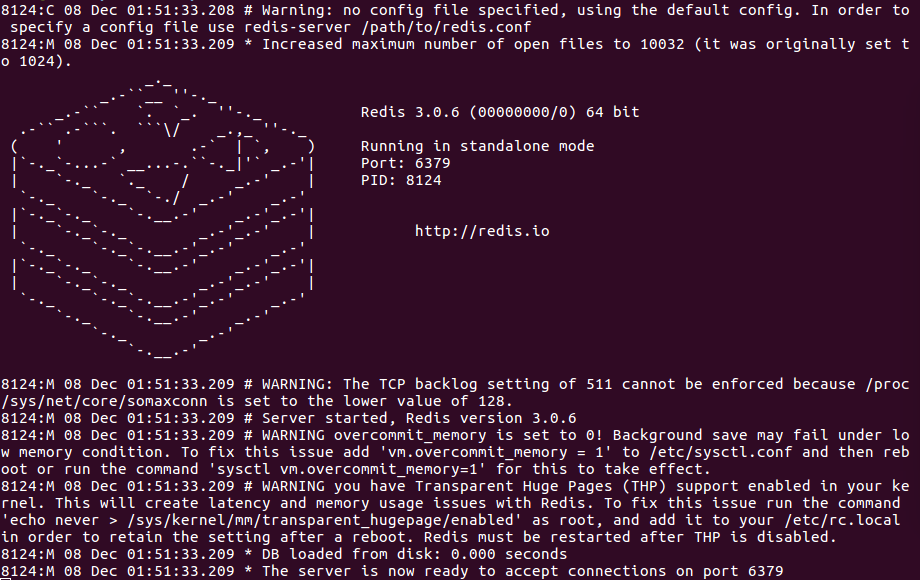
\includegraphics[scale=0.35]{server.png}
	\label{fig:server}
    \caption{Exemplo de um servidor Redis}
\end{figure}

Entre as estruturas suportadas pelo Redis temos:
\begin{itemize}
\item \textit{Strings}
\item \textit{Hashes}
\item \textit{Sets} e \textit{Sorted Sets}
\end{itemize}

As estruturas implementadas no Redis possuem algumas propriedas especiais:
\begin{itemize}
\item Armazenamento em disco, mesmo que elas estejam modificadas e armazenadas no servidor. Desta forma, REDIS é capaz de manter sua eficiencia.
Redis oferece opções comuns em banco de dados, como replicação, níveis de durabilidade mutáveis , etc.

\item A implementação de estruturas de dados geram \textit{stress} na memória, então, as estruturas de dados dentro do Redis provavelmente vai utilizar menos memória que as mesmas estruturas de dados dentro de linguagens de programação de alto nível.
\end{itemize}

Outra forma de se analizar o Redis é enchergá-lo como uma versão mais complexa de memchaced, onde as operações são apenas SET e GET. Redis no caso, possui dados mais complexos e mais operações possíveis também.

Várias linguagens possuem APIs dando suporte para Redis, incluindo: ActionScript, C, C++, C\#, Chicken Scheme, Clojure, Common Lisp, D, Dart, Erlang, Go, Haskell, Haxe, Io, Java, JavaScript (Node.js), Julia, Lua, Objective-C, OCaml, Perl, PHP, Pure Data, Python, R, Racket, Ruby, Rust, Scala, Smalltalk and Tcl.

Além disso, o Redis é utilizado por diversas companias muito conhecidas, como \textit{Twitter, GitHub, Weibo, Pinterest, Snapchat, Craigslist, Digg, StackOverflow} e \textit{Flickr}

\subsection{\textit{Publish/Subscribe}}

O modelo \textit{publish/subscribe} é um padrão de mensagens onde um remetente, chamado \textit{publisher} não programa as mensagens para serem enviadas para destinatários específicos, mas sim para canais de mensagem. Os destinatários, chamado \textit{subscribers} se inscrevem em determinado canal para receberem as mensagens.

Em vários sistemas \textit{publish/subscribe}, os remetentes mandam as mensagens para um \textit{broker}, que realiza a filtragem de mensagens.

Neste modelo, os remetentes não tem conhecimento dos inscritos, ou se ao menos eles existem. Desta forma, ambas as partes do modelo podem permanecer ignorantes da topologia do sistema, podendo dar continuidade às suas operações de maneira independente.

\subsubsection{\textit{Publish/Subscribe} no Redis}

As funções \textit{SUBSCRIBE}, \textit{UNSUBSCRIBE} e \textit{PUBLISH} são responsáveis pela implementação do paradigma \textit{Publish/Subscribe}. Por Exemplo, para se inscrever a um canal foo e bar, o cliente manda um comando \textit{SUBSCRIBE} dando o nome para os canais:
\begin{lstlisting}
SUBSCRIBE foo bar
\end{lstlisting}

Mensagens eviadas por outros clientes para esses canais serão enviados pelo Redis para todos os clientes inscritos.
Um cliente inscrito por um ou mais canais não devem enviar comandos, apesar de poderem se inscrever e cancelar a inscrição em outros canais. As respostas para estes comandos são enviados em forma de mensagens, para que o cliente possa ler as mensagens de forma coerente, o primeiro elemento da mensagem indica o tipo.

Formato das mensagens enviadas são:
\begin{itemize}
\item \textit{Subscribe} : significa que a inscrição ocorreu com sucesso dado pelo segundo elemento da mensagem. O terceiro elemento representa o numero de canais em que você está inscrito.
\item \textit{Unsubscribe} : significa que o cancelamento da inscrição ocorreu com sucesso dado pelo segundo elemento da mensagem. O terceiro elemento representa o numero de canais em que você está inscrito.
\item \textit{Message} : é a mensagem recebida como resultado de um comando \textit{PUBLISH} enviado por outro cliente. O segundo elemento é o nome do canal enviado, e o terceiro é a mensagem.  
\end{itemize}

\subsection{Redis Sentinel}

O \textit{Redis Sentinel} possibilita a disponibilidade do servidor Redis. Em termos práticos, significa que usando o \textit{Sentinel} pode criar resistência do servidor mesmo sem intervenção humana.

Essa sentinela também é capaz de cumprir outras tarefas como monitoramento, notificação e funciona como um provedor de configuração para os clientes.

A lista de capacidade do sentinela é definida:
\begin{itemize}
\item Monitoração: O sentinela constantemente checa se as instancias do Redis estão funcionando normalmente.
\item Notificação: A sentinela notifica o administrador do sistema, outros programas, a partir de uma API, que alguma coisa está errada com o Redis.
\item Recuperação: Se um mestre não está funcionando, a sentinela pode começar um processo de tornar um escravo para promove-lo para um mestre, reconfigurando os outros escravos para utilizar o novo mestre.
\item Configurador: A sentinela é um serviço de autoridade para os clientes, sendo que eles se conectam com a sentinela para perguntar o endereço do novo mestre.
\end{itemize}

O \textit{Redis Sentinel} é um sistema distribuído, ja que diversos processos estão cooperando entre sí com base na configuração dada dentro do sentinela,além disso, o \textit{Redis Sentinela} deve rodar em conjunto com o servidor Redis.

\section{Materiais e Métodos}
Nesta seção, serão descritos os detalhes de implementação na linguagem escolhida, a configuração do servidor Redis e a configuração do \textit{Redis Sentinel}.

\subsection{Redis .conf}

O arquivo redis.conf

\section{Resultados e Discusões}
\section{Conclusões}
\section{Referência}


\end{document}